\documentclass[12pt, a4paper]{article}

\usepackage{xcolor}	
 
%%%%%%%%%%%%%%%%%%%%%%%%%%%%%%%%%%%%%%%%%%%%%%%
% 				COLOURS
%%%%%%%%%%%%%%%%%%%%%%%%%%%%%%%%%%%%%%%%%%%%%%%

\definecolor{Red}{RGB}{128,0,0}
\definecolor{Blue}{RGB}{56,93,138}
\definecolor{Green}{RGB}{112,130,56}
\definecolor{Orange}{RGB}{255,133,50}
\definecolor{Magenta}{RGB}{139,0,139}
\definecolor{Brown}{RGB}{95,89,87}
\definecolor{Black}{RGB}{0,0,0}
\definecolor{White}{RGB}{255,255,255}
\definecolor{Gray}{RGB}{192,192,192}
%%%%%%%%%%%%%%%%%%%%%%%%%%%%%%%%%%%%%%%%%%%%%%%
% 				    MACROS
%%%%%%%%%%%%%%%%%%%%%%%%%%%%%%%%%%%%%%%%%%%%%%%

% Parentheses
\newcommand{\plbr}[1]	            { \left( #1 \right) }
\newcommand{\sqbr}[1]	            { \left[ #1 \right] }
\newcommand{\lcubr}[1]	            { \left\{ #1 \right.}

% Vectors and matrices
\newcommand{\cvvect}[1]	            { \begin{array}{c} #1 \end{array} }
\newcommand{\hvect}[2]	            { \begin{array}{ #1 } #2 \end{array} }
\newcommand{\matr}[2]	            { \begin{array}{ #1 } #2 \end{array} }

% Units
\newcommand{\unit}[1]				{ {\; \mathrm {#1}} }
\newcommand{\point}[1]				{ \mathsf{ #1 } }

% General notation
\newcommand{\ctime}					{ t }
\newcommand{\stepSize}				{ {\textrm d} \ctime}
\newcommand{\step}                  { k }


% Co-simulation notation - fundamentals
\newcommand{\state}					{ \mathbf{ x } }
\newcommand{\derivative}            { \dot{\state} }
\newcommand{\inputMod}				{ u }
\newcommand{\outputMod}				{ y }
\newcommand{\forceMod}				{ f }
\newcommand{\inputs}				{ \mathbf{\inputMod} }
\newcommand{\outputs}				{ \mathbf{\outputMod} }
\newcommand{\force}					{ \mathbf{\forceMod} }
\newcommand{\microstep}				{ h }
\newcommand{\communicationstep}		{ H }
\newcommand{\forceCorr}             { \tilde{\forceMod} }
\newcommand{\nextApproxInput}       { \tilde{\inputs} }

% Subscripts and superscripts
\newcommand{\trans}   				{ ^{\textrm T}}
\newcommand{\inv}   				{ ^{\textrm -1}}
\newcommand{\extr}   				{ ^{\textrm *}}


% Schemes
\newcommand{\angles}				{ \theta }
\newcommand{\cyldisplacement}		{ s_c }
\newcommand{\cylvelocity}			{ \dot{s}_c }
\newcommand{\discharge}				{ c_d }
\newcommand{\density}     			{ \rho }
\newcommand{\bulkMod}				{ \beta }
\newcommand{\outputValve}			{ a_o }
\newcommand{\inputValve}			{ a_i }
\newcommand{\compressibilityA}		{ a }
\newcommand{\compressibilityB}		{ b }
\newcommand{\spool}					{ \gamma }
\newcommand{\cyldisplacementIni}	{ s_c^0 }
\newcommand{\amplitude}				{ A }
\newcommand{\angular}				{ \omega }
\newcommand{\pressure}				{ p }
\newcommand{\power}                 { P }
\newcommand{\Residualpower}         { \delta \power }
\newcommand{\stiffness}				{ \kappa }
\newcommand{\damping}				{ c }
\newcommand{\mass}					{ m }
\newcommand{\length}				{ l }
\newcommand{\displacement}			{ \eta }
\newcommand{\velocity}				{ \dot{\eta} }
\newcommand{\acceleration}			{ \ddot{\eta} }
\newcommand{\piston}				{ a_p }
\newcommand{\matLO}					{ \bm{\Theta} }


% State-space - fundamentals
\newcommand{\stateMatrix}			{ \mathbf{A} }
\newcommand{\inputMatrix}			{ \mathbf{B} }
\newcommand{\outputMatrix}			{ \mathbf{C} }
\newcommand{\feedthrough}			{ \mathbf{D} }

% Matrices
\newcommand{\identity}				{ \mathbf{I} }
\newcommand{\zero}					{ \mathbf{0} }

% Estimadores
\newcommand{\estimation}            { \mathbf{X} }
\newcommand{\estimated}             { \mathbf{Y} }
\newcommand{\coefficient}           { \alpha}
\newcommand{\coefficients}          { \bm{\coefficient}}

\usepackage{tikz}

\usetikzlibrary{external}
\tikzexternalize

\begin{document}
	
%%%%%%%%%%%%%%%%%%%%%%%%%%%%%%%%%%%%%%%%% Double oscillator
	
\begin{figure}[ht!]\centering
	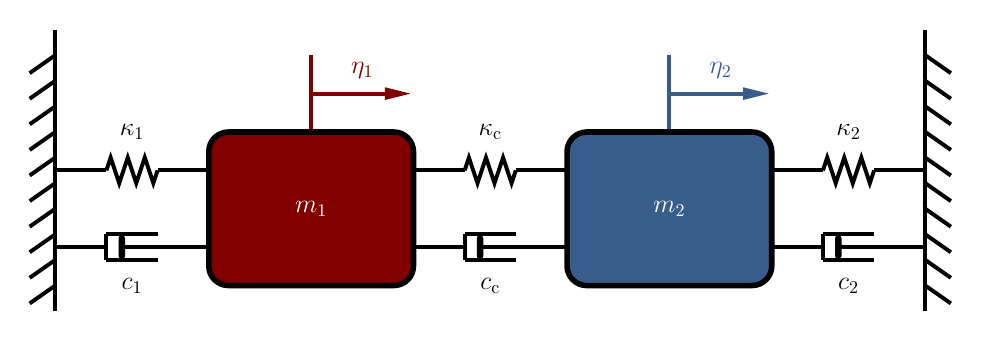
\begin{tikzpicture}[scale=0.65, transform shape] 
		
		% Axis
		\draw[-, draw=Red, line width=0.5mm] (-3.5,3) -- (-3.5,4.5);
		\draw[-, draw=Red, line width=0.5mm] (-3.5,3.75) -- (-2,3.75);
		\filldraw [fill=Red, draw=Red, line width=0.75mm] (-1.8,3.75) -- (-2,3.8) -- (-2,3.7) -- cycle;
		
		
		\draw[-, draw=Blue, line width=0.5mm] (3.5,3) -- (3.5,4.5);
		\draw[-, draw=Blue, line width=0.5mm] (3.5,3.75) -- (5,3.75);
		\filldraw [fill=Blue, draw=Blue, line width=0.75mm] (5.2,3.75) -- (5,3.8) -- (5,3.7) -- cycle;
		
		% Blocks
		\filldraw [fill=Red, draw=Black, rounded corners=0.25cm, line width=2pt] (-5.5,0) rectangle (-1.5,3);
		\filldraw [fill=Blue, draw=Black, rounded corners=0.25cm, line width=2pt] (1.5,0) rectangle (5.5,3);
		
		
		% Coupling
		\draw[-, draw=Black, line width=0.5mm] (-1.5,2.25) -- (-0.5,2.25);
		\draw[-, draw=Black, line width=0.5mm] (1.5,2.25) -- (0.5,2.25);
		\draw[-, draw=Black, line width=0.5mm] (-1.5,0.75) -- (-0.5,0.75);
		\draw[-, draw=Black, line width=0.5mm] (1.5,0.75) -- (-0.15,0.75);
		
		\draw[-, draw=Black, line width=0.5mm] (-0.5,1) -- (-0.5,0.5);
		\draw[-, draw=Black, line width=0.5mm] (-0.5,1) -- (0.5,1);
		\draw[-, draw=Black, line width=0.5mm] (-0.5,0.5) -- (0.5,0.5);
		\filldraw [fill=Black, draw=Black, rounded corners=0.05cm, line width=0.5pt] (-0.25,1) rectangle (-0.15,0.5);
		
		
		\draw[-, draw=Black, line width=0.5mm] (-0.5,2.25) -- (-0.4167,2.5) -- (-0.25,2) -- (-0.083,2.5) -- (0.083,2) -- (0.25,2.5) -- (0.4167,2)--(0.5,2.25);
		
		% Mass 1
		\draw[-, draw=Black, line width=0.5mm] (-8.5,2.25) -- (-7.5,2.25);
		\draw[-, draw=Black, line width=0.5mm] (-6.5,2.25) -- (-5.5,2.25);
		\draw[-, draw=Black, line width=0.5mm] (-8.5,0.75) -- (-7.5,0.75);
		\draw[-, draw=Black, line width=0.5mm] (-7.15,0.75) -- (-5.5,0.75);
		
		\draw[-, draw=Black, line width=0.5mm] (-7.5,1) -- (-7.5,0.5);
		\draw[-, draw=Black, line width=0.5mm] (-7.5,1) -- (-6.5,1);
		\draw[-, draw=Black, line width=0.5mm] (-7.5,0.5) -- (-6.5,0.5);
		\filldraw [fill=Black, draw=Black, rounded corners=0.05cm, line width=0.5pt] (-7.25,1) rectangle (-7.15,0.5);
		
		\draw[-, draw=Black, line width=0.5mm] (-7.5,2.25) -- (-7.4167,2.5) -- (-7.25,2) -- (-7.083,2.5) -- (-6.9167,2) -- (-6.75,2.5) -- (-6.5833,2)--(-6.5,2.25);
		
		
		% Mass 2
		\draw[-, draw=Black, line width=0.5mm] (8.5,2.25) -- (7.5,2.25);
		\draw[-, draw=Black, line width=0.5mm] (6.5,2.25) -- (5.5,2.25);
		\draw[-, draw=Black, line width=0.5mm] (8.5,0.75) -- (6.85,0.75);
		\draw[-, draw=Black, line width=0.5mm] (6.5,0.75) -- (5.5,0.75);
		
		\draw[-, draw=Black, line width=0.5mm] (6.5,1) -- (6.5,0.5);
		\draw[-, draw=Black, line width=0.5mm] (6.5,1) -- (7.5,1);
		\draw[-, draw=Black, line width=0.5mm] (6.5,0.5) -- (7.5,0.5);
		\filldraw [fill=Black, draw=Black, rounded corners=0.05cm, line width=0.5pt] (6.75,1) rectangle (6.85,0.5);
		
		\draw[-, draw=Black, line width=0.5mm] (6.5,2.25) -- (6.5833,2.5) -- (6.75,2) -- (6.9167,2.5) -- (7.0833,2) -- (7.25,2.5) -- (7.4167,2)--(7.5,2.25);
		
		% Grounds
		\draw[-, draw=Black, line width=0.5mm] (-8.5,-0.5) -- (-8.5,5);
		\draw[-, draw=Black, line width=0.5mm] (8.5,-0.5) -- (8.5,5);
		
		
		\draw[-, draw=Black, line width=0.5mm] (-8.5,4.5) -- (-9,4.15);
		\draw[-, draw=Black, line width=0.5mm] (-8.5,4) -- (-9,3.65);
		\draw[-, draw=Black, line width=0.5mm] (-8.5,3.5) -- (-9,3.15);
		\draw[-, draw=Black, line width=0.5mm] (-8.5,3) -- (-9,2.65);
		\draw[-, draw=Black, line width=0.5mm] (-8.5,2.5) -- (-9,2.15);
		\draw[-, draw=Black, line width=0.5mm] (-8.5,2) -- (-9,1.65);
		\draw[-, draw=Black, line width=0.5mm] (-8.5,1.5) -- (-9,1.15);
		\draw[-, draw=Black, line width=0.5mm] (-8.5,1) -- (-9,0.65);
		\draw[-, draw=Black, line width=0.5mm] (-8.5,0.5) -- (-9,0.15);
		\draw[-, draw=Black, line width=0.5mm] (-8.5,0) -- (-9,-0.35);
		
		
		\draw[-, draw=Black, line width=0.5mm] (8.5,4.5) -- (9,4.15);
		\draw[-, draw=Black, line width=0.5mm] (8.5,4) -- (9,3.65);
		\draw[-, draw=Black, line width=0.5mm] (8.5,3.5) -- (9,3.15);
		\draw[-, draw=Black, line width=0.5mm] (8.5,3) -- (9,2.65);
		\draw[-, draw=Black, line width=0.5mm] (8.5,2.5) -- (9,2.15);
		\draw[-, draw=Black, line width=0.5mm] (8.5,2) -- (9,1.65);
		\draw[-, draw=Black, line width=0.5mm] (8.5,1.5) -- (9,1.15);
		\draw[-, draw=Black, line width=0.5mm] (8.5,1) -- (9,0.65);
		\draw[-, draw=Black, line width=0.5mm] (8.5,0.5) -- (9,0.15);
		\draw[-, draw=Black, line width=0.5mm] (8.5,0) -- (9,-0.35);
		
		
		% Names
		\node[align=center, color = White, font=\Large] at (-35mm, 15mm) {$\mass_1$};
		\node[align=center, color = White, font=\Large] at (35mm, 15mm) {$\mass_2$};
		
		% Variables
		\node[align=center, color = Red, font=\Large] at (-25mm, 42mm) {$\displacement_1$};
		\node[align=center, color = Blue, font=\Large] at (45mm, 42mm) {$\displacement_2$};
		\node[align=center, color = Black, font=\Large] at (0mm, 30mm) {$\stiffness_{\rm c}$};
		\node[align=center, color = Black, font=\Large] at (0mm, 0mm) {$\damping_{\rm c}$};
		\node[align=center, color = Black, font=\Large] at (-70mm, 30mm) {$\stiffness_1$};
		\node[align=center, color = Black, font=\Large] at (-70mm, 0mm) {$\damping_1$};
		\node[align=center, color = Black, font=\Large] at (70mm, 30mm) {$\stiffness_2$};
		\node[align=center, color = Black, font=\Large] at (70mm, 0mm) {$\damping_2$};
		
	\end{tikzpicture} 
\end{figure}

\begin{figure}[ht!]\centering
	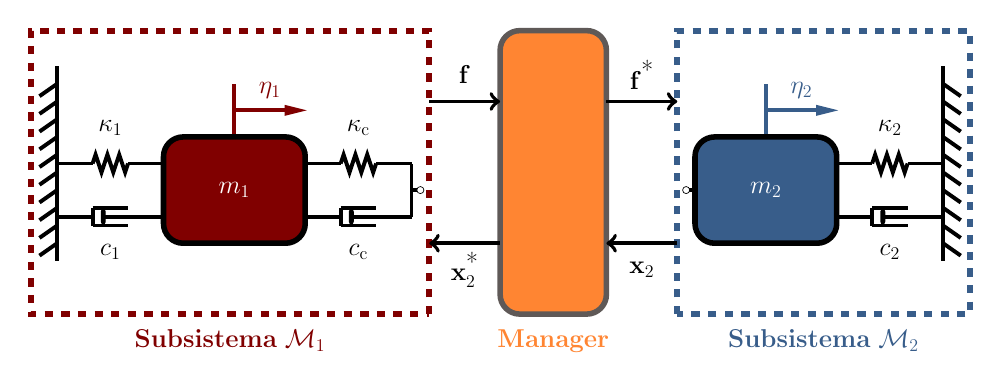
\begin{tikzpicture}[scale=0.45, transform shape] 
		
		% Axis
		\draw[-, draw=Red, line width=0.5mm] (-3.5,3) -- (-3.5,4.5);
		\draw[-, draw=Red, line width=0.5mm] (-3.5,3.75) -- (-2,3.75);
		\filldraw [fill=Red, draw=Red, line width=0.75mm] (-1.8,3.75) -- (-2,3.8) -- (-2,3.7) -- cycle;
		
		\draw[-, draw=Blue, line width=0.5mm] (11.5,3) -- (11.5,4.5);
		\draw[-, draw=Blue, line width=0.5mm] (11.5,3.75) -- (13,3.75);
		\filldraw [fill=Blue, draw=Blue, line width=0.75mm] (13.2,3.75) -- (13,3.8) -- (13,3.7) -- cycle;
		
		% Blocks
		\filldraw [fill=Red, draw=Black, rounded corners=0.25cm, line width=2pt] (-5.5,0) rectangle (-1.5,3);
		\filldraw [fill=Blue, draw=Black, rounded corners=0.25cm, line width=2pt] (9.5,0) rectangle (13.5,3);
		\filldraw [fill=Orange, draw=Brown, rounded corners=0.25cm, line width=2pt] (4,-2) rectangle (7,6);
		
		% Coupling
		\draw[-, draw=Black, line width=0.5mm] (-1.5,2.25) -- (-0.5,2.25);
		\draw[-, draw=Black, line width=0.5mm] (1.5,2.25) -- (0.5,2.25);
		\draw[-, draw=Black, line width=0.5mm] (-1.5,0.75) -- (-0.5,0.75);
		\draw[-, draw=Black, line width=0.5mm] (1.5,0.75) -- (-0.15,0.75);
		
		\draw[-, draw=Black, line width=0.5mm] (-0.5,1) -- (-0.5,0.5);
		\draw[-, draw=Black, line width=0.5mm] (-0.5,1) -- (0.5,1);
		\draw[-, draw=Black, line width=0.5mm] (-0.5,0.5) -- (0.5,0.5);
		\filldraw [fill=Black, draw=Black, rounded corners=0.05cm, line width=0.5pt] (-0.25,1) rectangle (-0.15,0.5);
		
		
		\draw[-, draw=Black, line width=0.5mm] (-0.5,2.25) -- (-0.4167,2.5) -- (-0.25,2) -- (-0.083,2.5) -- (0.083,2) -- (0.25,2.5) -- (0.4167,2)--(0.5,2.25);
		
		% Mass 1
		\draw[-, draw=Black, line width=0.5mm] (-8.5,2.25) -- (-7.5,2.25);
		\draw[-, draw=Black, line width=0.5mm] (-6.5,2.25) -- (-5.5,2.25);
		\draw[-, draw=Black, line width=0.5mm] (-8.5,0.75) -- (-7.5,0.75);
		\draw[-, draw=Black, line width=0.5mm] (-7.15,0.75) -- (-5.5,0.75);
		
		\draw[-, draw=Black, line width=0.5mm] (-7.5,1) -- (-7.5,0.5);
		\draw[-, draw=Black, line width=0.5mm] (-7.5,1) -- (-6.5,1);
		\draw[-, draw=Black, line width=0.5mm] (-7.5,0.5) -- (-6.5,0.5);
		\filldraw [fill=Black, draw=Black, rounded corners=0.05cm, line width=0.5pt] (-7.25,1) rectangle (-7.15,0.5);
		
		\draw[-, draw=Black, line width=0.5mm] (-7.5,2.25) -- (-7.4167,2.5) -- (-7.25,2) -- (-7.083,2.5) -- (-6.9167,2) -- (-6.75,2.5) -- (-6.5833,2)--(-6.5,2.25);
		
		\draw[-, draw=Black, line width=0.5mm] (1.5,0.75) -- (1.5,2.25);
		\draw[-, draw=Black, line width=0.5mm] (1.5,1.5) -- (1.75,1.5);
		\draw[fill=White, draw=Black, line width=0.25pt] (1.75,1.5) circle (1mm);
		
		% Mass 2
		\draw[-, draw=Black, line width=0.5mm] (15.5,2.25) -- (16.5,2.25);
		\draw[-, draw=Black, line width=0.5mm] (13.5,2.25) -- (14.5,2.25);
		\draw[-, draw=Black, line width=0.5mm] (16.5,0.75) -- (14.85,0.75);
		\draw[-, draw=Black, line width=0.5mm] (13.5,0.75) -- (14.5,0.75);
		
		\draw[-, draw=Black, line width=0.5mm] (14.5,1) -- (14.5,0.5);
		\draw[-, draw=Black, line width=0.5mm] (14.5,1) -- (15.5,1);
		\draw[-, draw=Black, line width=0.5mm] (14.5,0.5) -- (15.5,0.5);
		\filldraw [fill=Black, draw=Black, rounded corners=0.05cm, line width=0.5pt] (14.75,1) rectangle (14.85,0.5);
		
		\draw[-, draw=Black, line width=0.5mm] (14.5,2.25) -- (14.5833,2.5) -- (14.75,2) -- (14.9167,2.5) -- (15.0833,2) -- (15.25,2.5) -- (15.4167,2)--(15.5,2.25);
		
		\draw[-, draw=Black, line width=0.5mm] (9.5,1.5) -- (9.25,1.5);
		\draw[fill=White, draw=Black, line width=0.25pt] (9.25,1.5) circle (1mm);
		
		% Subsystems
		\draw [draw=Red, dashed, line width=0.75mm] (2,-2) -- (2,6) -- (-9.25,6) -- (-9.25,-2)-- cycle;
		\draw [draw=Blue, dashed, line width=0.75mm] (9,-2) -- (9,6) -- (17.25,6) -- (17.25,-2)-- cycle;
		
		% Grounds
		\draw[-, draw=Black, line width=0.5mm] (-8.5,-0.5) -- (-8.5,5);
		\draw[-, draw=Black, line width=0.5mm] (16.5,-0.5) -- (16.5,5);
		
		\draw[-, draw=Black, line width=0.5mm] (-8.5,4.5) -- (-9,4.15);
		\draw[-, draw=Black, line width=0.5mm] (-8.5,4) -- (-9,3.65);
		\draw[-, draw=Black, line width=0.5mm] (-8.5,3.5) -- (-9,3.15);
		\draw[-, draw=Black, line width=0.5mm] (-8.5,3) -- (-9,2.65);
		\draw[-, draw=Black, line width=0.5mm] (-8.5,2.5) -- (-9,2.15);
		\draw[-, draw=Black, line width=0.5mm] (-8.5,2) -- (-9,1.65);
		\draw[-, draw=Black, line width=0.5mm] (-8.5,1.5) -- (-9,1.15);
		\draw[-, draw=Black, line width=0.5mm] (-8.5,1) -- (-9,0.65);
		\draw[-, draw=Black, line width=0.5mm] (-8.5,0.5) -- (-9,0.15);
		\draw[-, draw=Black, line width=0.5mm] (-8.5,0) -- (-9,-0.35);
		
		\draw[-, draw=Black, line width=0.5mm] (16.5,4.5) -- (17,4.15);
		\draw[-, draw=Black, line width=0.5mm] (16.5,4) -- (17,3.65);
		\draw[-, draw=Black, line width=0.5mm] (16.5,3.5) -- (17,3.15);
		\draw[-, draw=Black, line width=0.5mm] (16.5,3) -- (17,2.65);
		\draw[-, draw=Black, line width=0.5mm] (16.5,2.5) -- (17,2.15);
		\draw[-, draw=Black, line width=0.5mm] (16.5,2) -- (17,1.65);
		\draw[-, draw=Black, line width=0.5mm] (16.5,1.5) -- (17,1.15);
		\draw[-, draw=Black, line width=0.5mm] (16.5,1) -- (17,0.65);
		\draw[-, draw=Black, line width=0.5mm] (16.5,0.5) -- (17,0.15);
		\draw[-, draw=Black, line width=0.5mm] (16.5,0) -- (17,-0.35);
		
		% Exchange
		\draw[->, draw=Black, line width=0.5mm] (2,4) -- (4,4);
		\draw[->, draw=Black, line width=0.5mm] (7,4) -- (9,4);
		\draw[<-, draw=Black, line width=0.5mm] (2,0) -- (4,0);
		\draw[<-, draw=Black, line width=0.5mm] (7,0) -- (9,0);
		
		\node[align=center, color = Black, font=\huge] 			at (30mm, 47.5mm) {$\force$};
		\node[align=center, color = Black, font=\huge] 			at (80mm, 47.5mm) {$\force\extr$};
		\node[align=center, color = Black, font=\huge] 			at (30mm, -7.5mm) {$\state_2\extr$};
		\node[align=center, color = Black, font=\huge] 			at (80mm, -7.5mm) {$\state_2$};
		
		% Names
		\node[align=center, color = White, font=\huge] at (-35mm, 15mm) {$\mass_1$};
		\node[align=center, color = White, font=\huge] at (115mm, 15mm) {$\mass_2$};
		
		% Variables
		\node[align=center, color = Red, font=\huge] at (-25mm, 43mm) {$\displacement_1$};
		\node[align=center, color = Blue, font=\huge] at (125mm, 43mm) {$\displacement_2$};
		\node[align=center, color = Black, font=\huge] at (0mm, 32.5mm) {$\stiffness_{\rm c}$};
		\node[align=center, color = Black, font=\huge] at (0mm, -2.5mm) {$\damping_{\rm c}$};
		\node[align=center, color = Black, font=\huge] at (-70mm, 32.5mm) {$\stiffness_1$};
		\node[align=center, color = Black, font=\huge] at (-70mm, -2.5mm) {$\damping_1$};
		\node[align=center, color = Black, font=\huge] at (150mm, 32.5mm) {$\stiffness_2$};
		\node[align=center, color = Black, font=\huge] at (150mm, -2.5mm) {$\damping_2$};
		
		\node[align=center, color = Red, font=\huge] 			at (-36.25mm, -27.5mm) {\textbf{Subsistema} $\mathcal{M}_1$};
		\node[align=center, color = Blue, font=\huge] 			at (131.25mm, -27.5mm) {\textbf{Subsistema} $\mathcal{M}_2$};
		\node[align=center, color = Orange, font=\huge] 			at (55mm, -27.5mm) {\textbf{Manager}};
		
		
	\end{tikzpicture} 
\end{figure}

%%%%%%%%%%%%%%%%%%%%%%%%%%%%%%%%%%%%%%%%% Hydraulic crane

\begin{figure}[ht!]\centering
	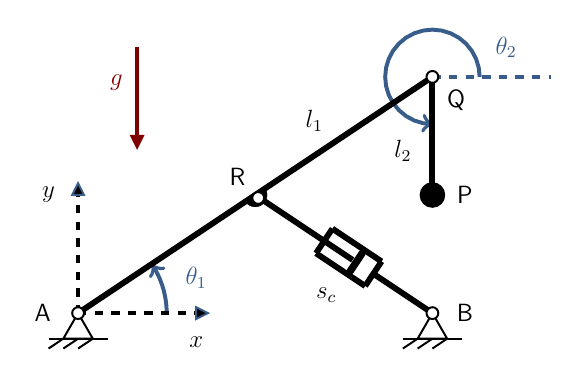
\begin{tikzpicture}[scale=0.75, transform shape] 
		
		% Supports
		\filldraw[-, fill=White, draw=Black, line width=0.25mm] (0,0) -- (-0.25,-0.433) -- (0.25,-0.433) -- cycle;
		
		\filldraw[-, fill=White, draw=Black, line width=0.25mm] (6,0) -- (5.75,-0.433) -- (6.25,-0.433) -- cycle;
		
		% Grounds
		\draw[-, draw=Black, line width=0.25mm] (-0.5,-0.433) -- (0.5,-0.433);
		
		\draw[-, draw=Black, line width=0.25mm] (0,-0.433) -- (-0.25,-0.6);
		\draw[-, draw=Black, line width=0.25mm] (0.25,-0.433) -- (0,-0.6);
		\draw[-, draw=Black, line width=0.25mm] (-0.25,-0.433) -- (-0.5,-0.6);
		
		\draw[-, draw=Black, line width=0.25mm] (5.5,-0.433) -- (6.5,-0.433);
		
		\draw[-, draw=Black, line width=0.25mm] (6,-0.433) -- (5.75,-0.6);
		\draw[-, draw=Black, line width=0.25mm] (6.25,-0.433) -- (6,-0.6);
		\draw[-, draw=Black, line width=0.25mm] (5.75,-0.433) -- (5.5,-0.6);
		
		% Gravity
		\draw[-, draw=Red, line width=0.5mm] (1,3) -- (1,4.5);
		\filldraw[-, fill=Red, draw=Red, line width=0.25mm] (1,2.8) -- (1.1,3) -- (0.9,3) -- cycle;
		\node[align=center, color = Red, font=\large] at (6.5mm, 39mm) {$g$};
		
		% Angles
		\node[align=center, color = Blue, font=\large] at (20mm, 6mm) {$\angles_1$};
		
		\node[align=center, color = Blue, font=\large] at (72.5mm, 45mm) {$\angles_2$};
		
		\draw[->, draw=Blue, line width=0.5mm, domain=0:33] plot({1.5*cos(\x)}, {1.5*sin(\x)});
		
		\draw[->, draw=Blue, line width=0.5mm, domain=0:270] plot({6+0.8*cos(\x)}, {4+0.8*sin(\x)});
		
		\draw[-, draw=Blue, dashed, line width=0.5mm] (6,4) -- (8,4);
		
		% Axis
		\draw[-, draw=Black, dashed, line width=0.5mm] (0,0) -- (0,2);
		\draw[-, draw=Black, dashed, line width=0.5mm] (0,0) -- (2,0);
		
		\filldraw[-, fill=Black, draw=Blue, line width=0.25mm] (0,2.2) -- (-0.1,2) -- (0.1,2) -- cycle;
		\filldraw[-, fill=Black, draw=Blue, line width=0.25mm] (2.2,0) -- (2,-0.1) -- (2,0.1) -- cycle;
		
		\node[align=center, color = Black, font=\large] at (20mm, -5mm) {$x$};
		\node[align=center, color = Black, font=\large] at (-5mm, 20mm) {$y$};
		
		% Rods
		\draw[-, draw=Black, line width=0.75mm] (0,0) -- (6,4);
		\draw[-, draw=Black, line width=0.75mm] (3,2) -- (4.65,0.9);
		\draw[-, draw=Black, line width=0.75mm] (5,0.667) -- (6,0);
		\draw[-, draw=Black, line width=0.75mm] (6,4) -- (6,2);
		\draw[fill=Black, draw=Black, line width=0.25mm] (6,2) circle (2mm);
		
		\filldraw[-, fill=Black, draw=Black, line width=0.05mm, domain=33.69:-146.31] plot({3+0.2*cos(\x)}, {2+0.2*sin(\x)});
		
		
		% Cylinder
		\draw[-, draw=Black, line width=0.75mm, ] (5.1387,0.8750) -- (4.8613,0.4589);
		\draw[-, draw=Black, line width=0.75mm, ] (5.1387,0.8750) -- (4.3066,1.4297);
		\draw[-, draw=Black, line width=0.75mm, ] (4.8613,0.4589) -- (4.0292,1.0137);
		\draw[-, draw=Black, line width=0.75mm, ] (4.3066,1.4297) -- (4.0292,1.0137);
		\filldraw [fill=Black, draw=Black, rounded corners=0.05cm, line width=0.5pt, rotate around ={-33.69:(4.75,0.833)}] (4.75,1.0833) rectangle (4.65,0.5833);
		
		% Joints
		\draw[fill=White, draw=Black, line width=0.25mm] (0,0) circle (1mm);
		\draw[fill=White, draw=Black, line width=0.25mm] (6,4) circle (1mm);
		\draw[fill=White, draw=Black, line width=0.25mm] (6,0) circle (1mm);
		\draw[fill=White, draw=Black, line width=0.25mm] (3.05,1.95) circle (1mm);
		
		% Variables
		\node[align=center, color = Black, font=\large] at (-6mm, 0mm) {$\point{A}$};
		\node[align=center, color = Black, font=\large] at (64mm, 36mm) {$\point{Q}$};
		\node[align=center, color = Black, font=\large] at (65.5mm, 20mm) {$\point{P}$};
		\node[align=center, color = Black, font=\large] at (27mm, 23mm) {$\point{R}$};
		\node[align=center, color = Black, font=\large] at (65.5mm, 0mm) {$\point{B}$};
		
		\node[align=center, color = Black, font=\large] at (40mm, 32.5mm) {$\length_1$};
		\node[align=center, color = Black, font=\large] at (55mm, 27.5mm) {$\length_2$};
		\node[align=center, color = Black, font=\large] at (42mm, 3mm) {$\cyldisplacement$};
		
	\end{tikzpicture} 
\end{figure}

\begin{figure}[ht!]\centering
	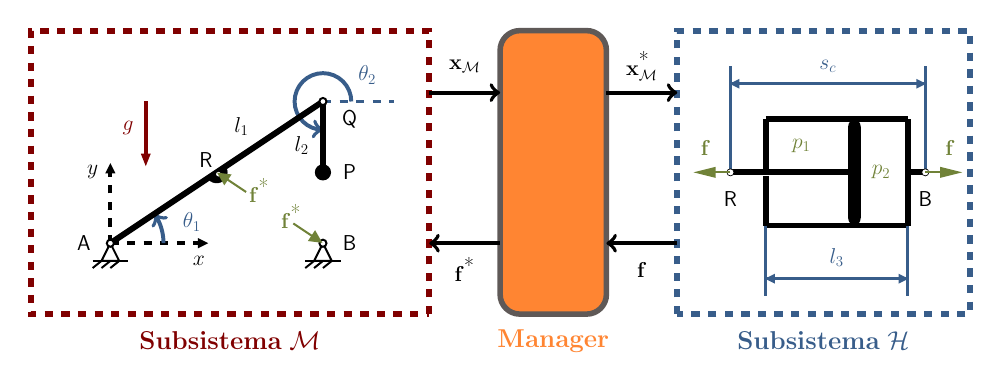
\begin{tikzpicture}[scale=0.45, transform shape] 
		
		% Blocks
		\filldraw [fill=Orange, draw=Brown, rounded corners=0.25cm, line width=2pt] (4,-2) rectangle (7,6);
		
		% Axis
		\draw[-, draw=Black, line width=0.5mm, dashed] (-7,0) -- (-7,2);
		\draw[-, draw=Black, line width=0.5mm, dashed] (-7,0) -- (-4.5,0);
		\filldraw[-, fill=Black, draw=Black, line width=0.25mm] (-7,2.2) -- (-7.1,2) -- (-6.9,2) -- cycle;
		\filldraw[-, fill=Black, draw=Black, line width=0.25mm] (-4.3,0) -- (-4.5,0.1) -- (-4.5,-0.1) -- cycle;
		\node[align=center, color = Black, font=\LARGE] at (-45mm, -5mm) {$x$};
		\node[align=center, color = Black, font=\LARGE] at (-75mm, 20 mm) {$y$};
		
		% Gravity
		\draw[-, draw=Red, line width=0.5mm] (-6,4) -- (-6,2.5);
		\filldraw[-, fill=Red, draw=Red, line width=0.25mm] (-6.1,2.5) -- (-5.9,2.5) -- (-6,2.25) -- cycle;
		\node[align=center, color = Red, font=\LARGE] at (-65mm, 32.5mm) {$g$};
		
		% Angles
		\node[align=center, color = Blue, font=\LARGE] at (-47mm, 6mm) {$\angles_1$};
		\node[align=center, color = Blue, font=\LARGE] at (2.5mm, 47.5mm) {$\angles_2$};
		
		\draw[->, draw=Blue, line width=0.5mm, domain=0:33] plot({1.5*cos(\x)-7}, {1.5*sin(\x)});
		\draw[->, draw=Blue, line width=0.5mm, domain=0:270] plot({-1+0.8*cos(\x)}, {4+0.8*sin(\x)});
		\draw[-, draw=Blue, dashed, line width=0.5mm] (-1,4) -- (1,4);
		
		% Crane
		\filldraw[-, fill=White, draw=Black, line width=0.25mm] (-7,0) -- (-7.25,-0.5) -- (-6.75,-0.5) -- cycle;
		\draw[-, draw=Black, line width=0.25mm] (-7.5,-0.5) -- (-6.5,-0.5);
		\draw[-, draw=Black, line width=0.25mm] (-7,-0.5) -- (-7.25,-0.7);
		\draw[-, draw=Black, line width=0.25mm] (-7.25,-0.5) -- (-7.5,-0.7);
		\draw[-, draw=Black, line width=0.25mm] (-6.75,-0.5) -- (-7,-0.7);
		
		\filldraw[-, fill=White, draw=Black, line width=0.25mm] (-1,0) -- (-1.25,-0.5) -- (-0.75,-0.5) -- cycle;
		\draw[-, draw=Black, line width=0.25mm] (-0.5,-0.5) -- (-1.5,-0.5);
		\draw[-, draw=Black, line width=0.25mm] (-1,-0.5) -- (-1.25,-0.7);
		\draw[-, draw=Black, line width=0.25mm] (-1.25,-0.5) -- (-1.5,-0.7);
		\draw[-, draw=Black, line width=0.25mm] (-0.75,-0.5) -- (-1,-0.7);
		
		\draw[-, draw=Black, line width=0.75mm] (-7,0) -- (-1,4);
		%	\draw[-, draw=Black, line width=0.75mm, rotate around={-33.69:(-4, 2)}] (-4,2) -- (-3.2,2);
		%	\draw[-, draw=Black, line width=0.75mm, rotate around={-33.69:(-4, 2)}] (-1.2,2) -- (-0.4,2);
		\draw[-, draw=Black, line width=0.75mm] (-1,4) -- (-1,2);
		\filldraw[-, fill=Black, draw=Black, line width=0.05mm, domain=33.69:-146.31] plot({-4+0.3*cos(\x)}, {2+0.3*sin(\x)});
		
		
		\draw[fill=Black, draw=Black, line width=0.25mm] (-1,2) circle (2mm);
		\draw[fill=White, draw=Black, line width=0.25mm] (-7,0) circle (1mm);
		\draw[fill=White, draw=Black, line width=0.25mm] (-1,4) circle (1mm);
		\draw[fill=White, draw=Black, line width=0.25mm] (-1,0) circle (1mm);
		\draw[fill=White, draw=Black, line width=0.25mm] (-3.95,1.95) circle (1mm);
		
		%	\draw[fill=White, draw=Black, line width=0.25pt, rotate around={-33.69:(-4, 2)}] (-3.2,2) circle (1mm);
		%	\draw[fill=White, draw=Black, line width=0.25pt, rotate around={-33.69:(-4, 2)}] (-1.2,2) circle (1mm);
		
		\draw[-, draw=Green, line width=0.25mm, rotate around={-33.69:(-4, 2)}] (-3.8,2) -- (-3,2);
		\draw[-, draw=Green, line width=0.25mm, rotate around={-33.69:(-4, 2)}] (-1.4,2) -- (-0.5,2);
		\filldraw [fill=Green, draw=Green, line width=0.75mm, rotate around={-33.69:(-4, 2)}] (-3.8,2) -- (-3.7,2.05) -- (-3.7,1.95) -- cycle;
		\filldraw [fill=Green, draw=Green, line width=0.75mm, rotate around={-33.69:(-4, 2)}] (-0.6,2) -- (-0.7,2.05) -- (-0.7,1.95) -- cycle;
		
		
		% Piston
		\filldraw [fill=Black, draw=Black, rounded corners=0.1cm, line width=0.75pt] (13.85,3.5) rectangle (14.15,0.5);
		\draw[-, line width=0.75mm] (10.5,2) -- (14,2);
		
		\draw[-, line width=0.75mm] (11.5,2.1) -- (11.5,3.5);
		\draw[-, line width=0.75mm] (11.5,1.9) -- (11.5,0.5);
		\draw[-, line width=0.75mm] (11.5,0.5) -- (15.5,0.5);
		\draw[-, line width=0.75mm] (11.5,3.5) -- (15.5,3.5);
		\draw[-, line width=0.75mm] (15.5,3.5) -- (15.5,0.5);
		\draw[-, line width=0.75mm] (15.5,2) -- (16,2);
		
		\draw[-, draw=Blue, line width=0.4mm] (11.5,0.5) -- (11.5,-1.5);
		\draw[-, draw=Blue, line width=0.4mm] (15.5,0.5) -- (15.5,-1.5);
		\draw[-, draw=Blue, line width=0.4mm] (11.5,-1) -- (15.5,-1);
		\filldraw[fill = Blue, draw=Blue, line width=0.5mm] (11.6,-1) -- (11.7,-0.95) -- (11.7,-1.05) -- cycle;
		\filldraw[fill = Blue, draw=Blue, line width=0.5mm] (15.4,-1) -- (15.3,-0.95) -- (15.3,-1.05) -- cycle;
		
		\draw[-, draw=Blue, line width=0.4mm] (10.5,2) -- (10.5,5);
		\draw[-, draw=Blue, line width=0.4mm] (16,2) -- (16,5);
		\draw[-, draw=Blue, line width=0.4mm] (10.5,4.5) -- (16,4.5);
		\filldraw[fill = Blue, draw=Blue, line width=0.5mm] (10.6,4.5) -- (10.7,4.45) -- (10.7,4.55) -- cycle;
		\filldraw[fill = Blue, draw=Blue, line width=0.5mm] (15.9,4.5) -- (15.8,4.45) -- (15.8,4.55) -- cycle;
		
		\draw[fill=White, draw=Black, line width=0.25pt] (10.5,2) circle (1mm);
		\draw[fill=White, draw=Black, line width=0.25pt] (16,2) circle (1mm);
		
		\draw[-, draw=Green, line width=0.25mm] (10.5,2) -- (10,2);
		\draw[-, draw=Green, line width=0.25mm] (16.5,2) -- (16,2);
		\filldraw [fill=Green, draw=Green, line width=0.75mm] (16.7,2) -- (16.5,2.05) -- (16.5,1.95) -- cycle;
		\filldraw [fill=Green, draw=Green, line width=0.75mm] (9.8,2) -- (10,2.05) -- (10,1.95) -- cycle;
		
		% Subsystems
		\draw [draw=Red, dashed, line width=0.75mm] (2,-2) -- (2,6) -- (-9.25,6) -- (-9.25,-2)-- cycle;
		\draw [draw=Blue, dashed, line width=0.75mm] (9,-2) -- (9,6) -- (17.25,6) -- (17.25,-2)-- cycle;
		
		% Exchange
		\draw[->, draw=Black, line width=0.5mm] (2,4.25) -- (4,4.25);
		\draw[->, draw=Black, line width=0.5mm] (7,4.25) -- (9,4.25);
		\draw[<-, draw=Black, line width=0.5mm] (2,0) -- (4,0);
		\draw[<-, draw=Black, line width=0.5mm] (7,0) -- (9,0);
		
		\node[align=center, color = Black, font=\LARGE] 			at (30mm, -7.5mm) {$\force\extr$};
		\node[align=center, color = Black, font=\LARGE] 			at (80mm, -7.5mm) {$\force$};
		\node[align=center, color = Black, font=\LARGE] 			at (80mm, 50mm) {$\state_\mathcal{M}\extr$};
		\node[align=center, color = Black, font=\LARGE] 			at (30mm, 50mm) {$\state_\mathcal{M}$};
		
		% Variables
		\node[align=center, color = Green, font=\LARGE] 			at (125mm, 27.5mm) {$\pressure_1$};
		\node[align=center, color = Green, font=\LARGE] 			at (147.5mm, 20mm) {$\pressure_2$};
		\node[align=center, color = Blue, font=\LARGE] 			at (135mm, -4mm) {$\length_3$};
		\node[align=center, color = Blue, font=\LARGE] 			at (132.5mm, 50mm) {$\cyldisplacement$};
		
		\node[align=center, color = Green, font=\LARGE] 			at (167mm, 27mm) {$\force$};
		\node[align=center, color = Green, font=\LARGE] 			at (98mm, 27mm) {$\force$};
		\node[align=center, color = Green, font=\LARGE] 			at (-28mm, 15mm) {$\force\extr$};
		\node[align=center, color = Green, font=\LARGE] 			at (-19mm, 7.5mm) {$\force\extr$};
		
		\node[align=center, color = Black, font=\LARGE] at (-77.5mm, 0mm) {$\point{A}$};
		\node[align=center, color = Black, font=\LARGE] at (-2.5mm, 35mm) {$\point{Q}$};
		\node[align=center, color = Black, font=\LARGE] at (-43mm, 23.5mm) {$\point{R}$};
		\node[align=center, color = Black, font=\LARGE] at (-2.5mm, 20mm) {$\point{P}$};
		\node[align=center, color = Black, font=\LARGE] at (-2.5mm, 0mm) {$\point{B}$};
		
		\node[align=center, color = Black, font=\LARGE] at (105mm, 12.5mm) {$\point{R}$};
		\node[align=center, color = Black, font=\LARGE] at (160mm, 12.5mm) {$\point{B}$};
		
		\node[align=center, color = Black, font=\LARGE] at (-33mm, 33mm) {$\length_1$};
		\node[align=center, color = Black, font=\LARGE] at (-16mm, 27.5mm) {$\length_2$};
		
		% Names
		\node[align=center, color = Red, font=\huge] 			at (-36.25mm, -27.5mm) {\textbf{Subsistema} $\mathcal{M}$};
		\node[align=center, color = Blue, font=\huge] 			at (131.25mm, -27.5mm) {\textbf{Subsistema} $\mathcal{H}$};
		\node[align=center, color = Orange, font=\huge] 			at (55mm, -27.5mm) {\textbf{Manager}};
		
	\end{tikzpicture}
\end{figure}

\begin{figure}[ht!]\centering
	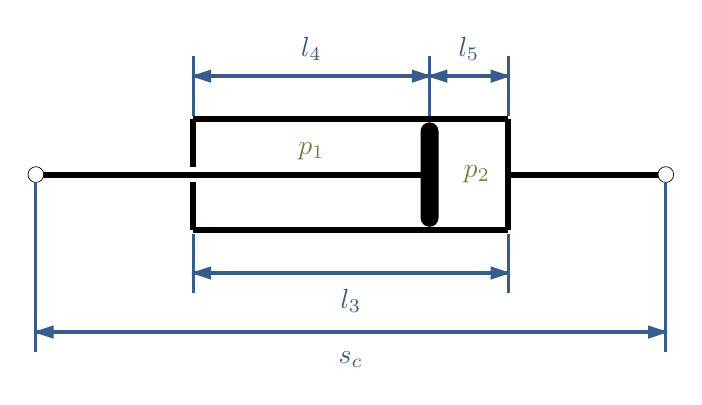
\begin{tikzpicture}[scale=1.0, transform shape] 
		
		% Piston
		\filldraw [fill=Black, draw=Black, rounded corners=0.1cm, line width=0.75pt] (-0.1,-0.65) rectangle (0.1,0.65);
		\draw[-, line width=0.75mm] (-5,0) -- (0,0);
		
		% Cylinder
		\draw[-, line width=0.75mm] (-3,0.7) -- (1,0.7);
		\draw[-, line width=0.75mm] (-3,-0.7) -- (1,-0.7);
		\draw[-, line width=0.75mm] (1,0.7) -- (1,-0.7);
		\draw[-, line width=0.75mm] (1,0) -- (3,0);
		\draw[-, line width=0.75mm] (-3,0.7) -- (-3,0.1);
		\draw[-, line width=0.75mm] (-3,-0.7) -- (-3,-0.1);
		
		% Text
		\node[align=center, color = Green] 			at (-15mm, 3mm) {$\pressure_1$};
		\node[align=center, color = Green] 			at (6mm, 0mm) {$\pressure_2$};
		
		% Circles
		\draw[fill=White, draw=Black, line width=0.25pt] (3,0) circle (1mm);
		\draw[fill=White, draw=Black, line width=0.25pt] (-5,0) circle (1mm);
		
		% Dimensions
		\draw[-, draw=Blue, line width=0.4mm] (-3,0.75) -- (-3,1.5);
		\draw[-, draw=Blue, line width=0.4mm] (0,0.75) -- (0,1.5);
		\draw[-, draw=Blue, line width=0.4mm] (1,0.75) -- (1,1.5);
		
		\draw[-, draw=Blue, line width=0.4mm] (-3,-0.75) -- (-3,-1.5);
		\draw[-, draw=Blue, line width=0.4mm] (1,-0.75) -- (1,-1.5);
		
		\draw[-, draw=Blue, line width=0.4mm] (-5,-0.1) -- (-5,-2.25);
		\draw[-, draw=Blue, line width=0.4mm] (3,-0.1) -- (3,-2.25);
		
		% Dimensions
		\draw[-, draw=Blue, line width=0.5mm] (-3,1.25) to (0,1.25);
		\draw[-, draw=Blue, line width=0.5mm] (0,1.25) to (1,1.25);
		\draw[-, draw=Blue, line width=0.5mm] (-3,-1.25) to (1,-1.25);
		\draw[-, draw=Blue, line width=0.5mm] (-5,-2) to (3,-2);
		
		% Arrows
		\filldraw[fill = Blue, draw=Blue, line width=0.5mm] (-2.95,1.25) -- (-2.8,1.2) -- (-2.8,1.3) -- cycle;
		\filldraw[fill = Blue, draw=Blue, line width=0.5mm] (-0.05,1.25) -- (-0.2,1.2) -- (-0.2,1.3) -- cycle;
		
		\filldraw[fill = Blue, draw=Blue, line width=0.5mm] (0.05,1.25) -- (0.2,1.2) -- (0.2,1.3) -- cycle;
		\filldraw[fill = Blue, draw=Blue, line width=0.5mm] (0.95,1.25) -- (0.8,1.2) -- (0.8,1.3) -- cycle;
		
		\filldraw[fill = Blue, draw=Blue, line width=0.5mm] (-2.95,-1.25) -- (-2.8,-1.2) -- (-2.8,-1.3) -- cycle;
		\filldraw[fill = Blue, draw=Blue, line width=0.5mm] (0.95,-1.25) -- (0.8,-1.2) -- (0.8,-1.3) -- cycle;
		
		\filldraw[fill = Blue, draw=Blue, line width=0.5mm] (-4.95,-2) -- (-4.8,-1.95) -- (-4.8,-2.05) -- cycle;
		\filldraw[fill = Blue, draw=Blue, line width=0.5mm] (2.95,-2) -- (2.8,-1.95) -- (2.8,-2.05) -- cycle;
		
		% Vars
		\node[align=center, color = Blue] 			at (-15mm, 16mm) {$\length_4$};
		\node[align=center, color = Blue] 			at (5mm, 16mm) {$\length_5$};
		\node[align=center, color = Blue] 			at (-10mm, -16mm) {$\length_3$};
		\node[align=center, color = Blue] 			at (-10mm, -23.5mm) {$\cyldisplacement$};
		
	\end{tikzpicture}
\end{figure}


\end{document}